\documentclass[]{tufte-handout}

% ams
\usepackage{amssymb,amsmath}

\usepackage{ifxetex,ifluatex}
\usepackage{fixltx2e} % provides \textsubscript
\ifnum 0\ifxetex 1\fi\ifluatex 1\fi=0 % if pdftex
  \usepackage[T1]{fontenc}
  \usepackage[utf8]{inputenc}
\else % if luatex or xelatex
  \makeatletter
  \@ifpackageloaded{fontspec}{}{\usepackage{fontspec}}
  \makeatother
  \defaultfontfeatures{Ligatures=TeX,Scale=MatchLowercase}
  \makeatletter
  \@ifpackageloaded{soul}{
     \renewcommand\allcapsspacing[1]{{\addfontfeature{LetterSpace=15}#1}}
     \renewcommand\smallcapsspacing[1]{{\addfontfeature{LetterSpace=10}#1}}
   }{}
  \makeatother

\fi

% graphix
\usepackage{graphicx}
\setkeys{Gin}{width=\linewidth,totalheight=\textheight,keepaspectratio}

% booktabs
\usepackage{booktabs}

% url
\usepackage{url}

% hyperref
\usepackage{hyperref}

% units.
\usepackage{units}


\setcounter{secnumdepth}{-1}

% citations


% pandoc syntax highlighting

% longtable

% multiplecol
\usepackage{multicol}

% strikeout
\usepackage[normalem]{ulem}

% morefloats
\usepackage{morefloats}


% tightlist macro required by pandoc >= 1.14
\providecommand{\tightlist}{%
  \setlength{\itemsep}{0pt}\setlength{\parskip}{0pt}}

% title / author / date
\title{PlanGobiernos\_2021}
\author{LZ}
\date{1/22/2021}


\begin{document}

\maketitle




\#Planes de Gobierno: Un análisis de texto

\hypertarget{introducciuxf3n}{%
\subsection{Introducción}\label{introducciuxf3n}}

Aquí se leen los planes de gobierno en PDF descargados de la página

\#Planes de Gobierno: Un análisis de Texto

\#\#Introducción

Me la pelan

\begin{verbatim}
## # A tibble: 10 x 2
##    word           n
##    <chr>      <int>
##  1 nacional     935
##  2 desarrollo   785
##  3 salud        733
##  4 sistema      660
##  5 servicios    481
##  6 gobierno     466
##  7 nivel        446
##  8 social       410
##  9 recursos     331
## 10 acceso       326
\end{verbatim}

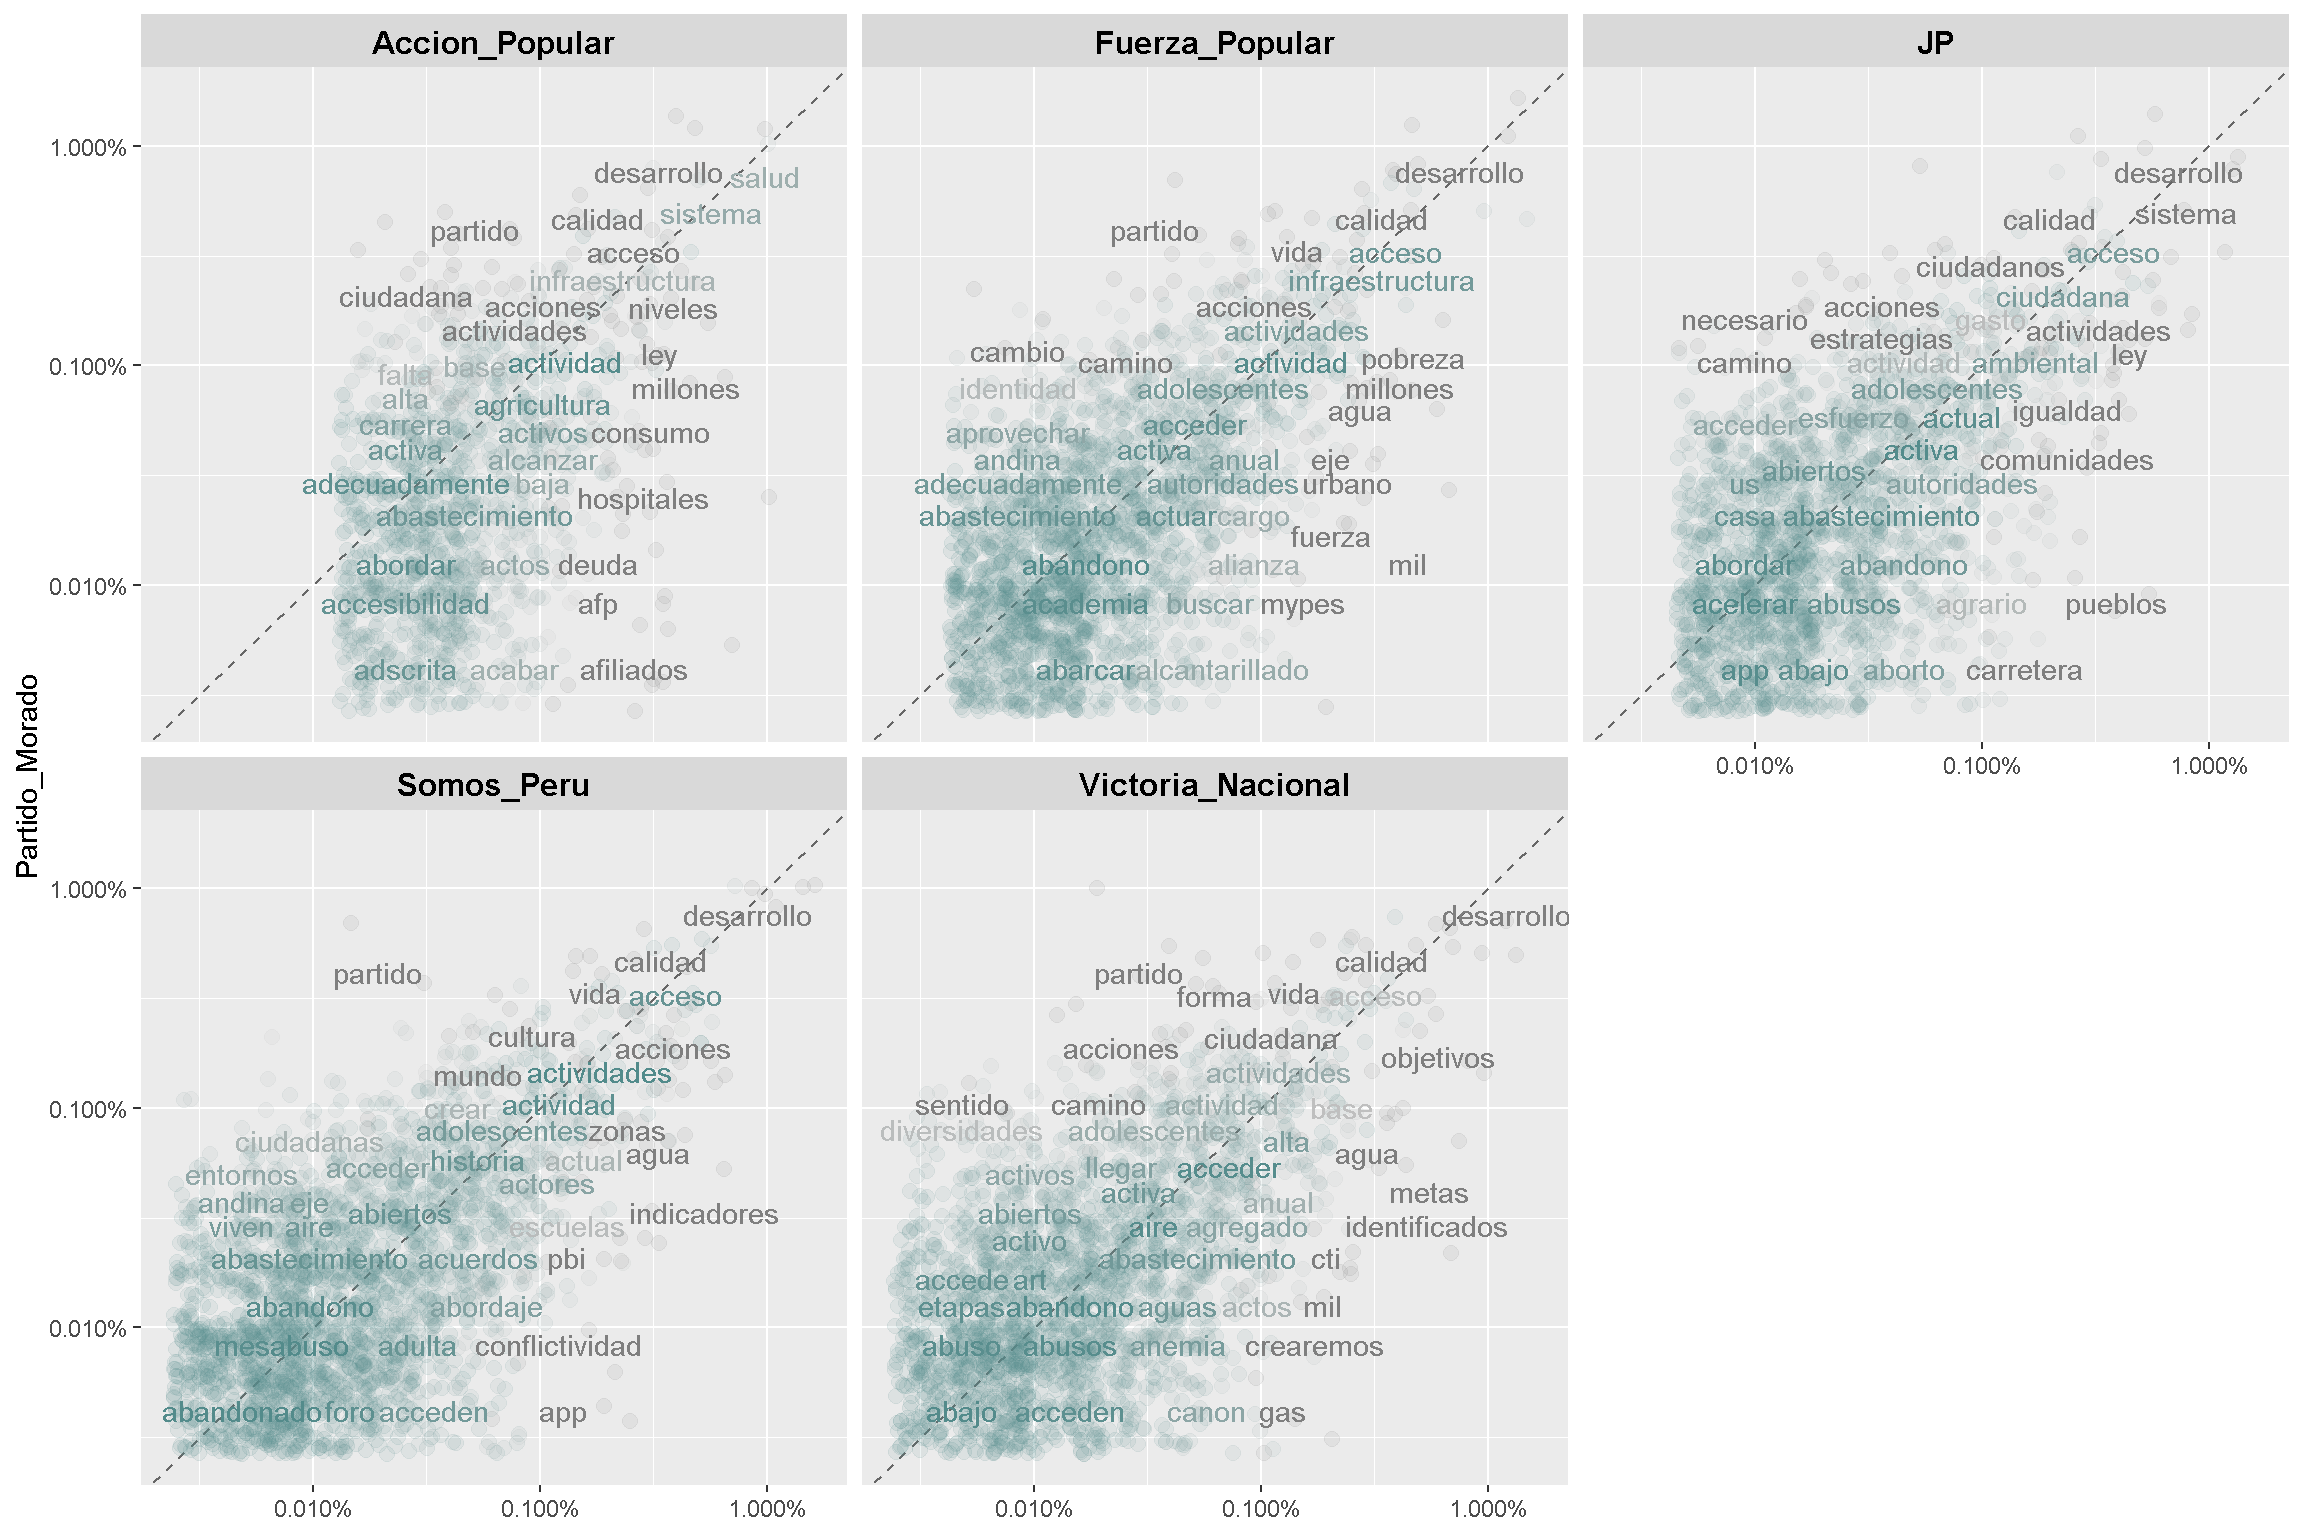
\includegraphics{Figs/unnamed-chunk-5-1}



\end{document}
